The second iteration of design utilises a control theory concept of
\emph{Proportional}, \emph{Integral} and \emph{Derivative} (PID) controllers. PID controllers
provide the ability to regulate control continuously throughout the
runtime of the application. Testing of this phase is conducted on a 4-CPU and 8-CPU Linux Xenial virtual machine. The benchmark used for testing
is DaCapo benchmarks \cite{blackburn2006dacapo}, as described in
Chapter 3. 
\newline\newline
The findings indicate that there is improved control over GC
utilisation compared to \emph{CatNap} results and the original JVM. There is
also better performance as well.
\newline\newline
The phase is called \emph{Circling} as it involves constant movements that
result in the GC adjusting its resource usage. This constant movement is
similar to a cat that circles round on a bed to find the
 most comfortable position.
\subsection{Approach}
The overall approach used for the PID controller is to develop a
separate PID controller for each of the three variables: heap size, the
number of GC threads and interval between local GCs. This approach is
used because the literature and much of the research on PID controllers
focus on single input and single output systems, such as White et al.`s
(2013). The concept of a PID controller is described in Chapter 2, and it allows for
more dynamic adjustments to a system. Using a PID controller reduces the
likelihood of a system crossing set boundaries. Generally, the PID
controller involves exponential calculations to avoid integral windup,
i.e., the integral factor based on past errors continually increases.
However, an attempt is made to avoid calculations that require importing
any additional math header files to ensure the overhead of the mode is minimised where possible. Instead, only the math header files
currently part of the OpenJ9 JVM are within scope. Thus, some
calculations are simplified to avoid the use of exponential functions.

\subsection{Implementation}
The PID controller is implemented using several structs. This
implementation included some refactoring of the initial structs created
in \emph{CatNap}. Firstly, a \verb|pidControl| struct is added. This struct calculates
each PID component for each variable. The same error is used for all
variables. The variables contained within the \verb|pidControl| struct include
the constants for each component, the integral sum, the number of previous
errors in the sliding window and the final output from the PID. All of the
struct variables are of type \verb|double| to allow decimal point PID adjustments.
However, the adjustments are rounded up before the actual variables are
changed. Following from White et al. (2013), a sliding window approach
is used to calculate the integral sum. This approach is used as most of
the OpenJ9/OMR code does not use array-like structures unless necessary.
In addition, an integral sum comprising of a single variable for the sum and a variable for the number of items in the window is easier to use within the OpenJ9/OMR code. The maximum number of items in the window is set to 5, similar
to White et al. (2013). The constants for each component are set within
the \emph{ParallelDispatcher}. There is an individual constant for each
variable (heap size, number of GC threads and interval between local
GCs) allowing the ability to set a different value for each. This
individual constant is not utilised in the testing as the main aim of
\emph{Circling} is to identify whether the PID controller is an excellent
choice for reducing GC utilisation and the ideal relationship between
\emph{Proportional}, \emph{Integral} and \emph{Derivative} values.
\newline\newline
The second struct added is \verb|gcMonitoring|. This struct incorporates the
monitoring of GC utilisation from the original \verb|gcElastic| struct. The
reasoning behind making a new struct is that it made the functionality
of the new mode clearer. Without the \verb|gcMonitoring| struct, all of the
variables needed to monitor GC would be included with the variables
being adjusted. Finally, the \verb|gcElastic| struct added two new variables:
\verb|heapSizeTarget| and \verb|gcIntervalTarget|. These two variables are necessary
because the adjustments calculated through the PID controller do not
take immediate effect for heap size or the interval between local GCs.
Instead, there is a delay until the code for heap size and the interval
is executed.
\newline\newline
Within the actual logic of the PID controller, the following steps were
followed
\begin{enumerate}
\def\labelenumi{\arabic{enumi}.}
\item
  Calculate GC utilisation.
\item
  Calculate error.
\item
  Calculate proportional values.
\item
  Calculate integral sum.
\item
  Calculate integral values.
\item
  Calculate derivative values.
\item
  Calculate the final impact of proportional, integral and derivative
  values.
\item
  If the output is valid then adjust the variables or the target
  variables.
\end{enumerate}
Step 3 to 8 were repeated for each variable (heap size, number of GC threads and interval between local GCs). These steps are expressible in equations as well, which are provided below.
\newline\newline
\begin{math}[H]
(1)\    E_{t} \ =\ GC_{target} \ -GC_{actual}\\
(2)\     P_{t} \ =\ P_{k} \ *\ E_{t}\\
(3)\ I_{s} =\sum\limits _{t} E_{t} \ *\ T_{t}\\
(4)\ I_{t} \ =\ I_{s\ } *\ I_{k}\\
(5)\ D_{temp} \ =\ \frac{( E_{t} \ -\ E_{t\ -1})}{T_{t}}\\
(6)\ D_{t} \ =\ D_{temp} \ *\ D_{k}\\
(7)\ Heap\ =\ D_{t} \ +\ I_{t} \ +P_{t}
\end{math}
\newline\newline
The first equation represents the calculation for the current error at time \emph{t}. This equation relates to step 2 in the above list. The target GC utilisation is set to 5 times the number of CPUs meaning that the mode adjusts depending on the size of the virtual machine.  The second equation calculates the proportional value by multiplying a set proportional constant (\begin{math}{P_{k}}\end{math}). Equation 3 sums up the error at time \emph{t}. This summing of the error occurs if the size of the sliding window is less than 5. Otherwise, the sum is set to 0, and the process begins next GC. Equation 4 uses the sum calculated in the third equation and multiplies it by an integral constant (\begin{math} {I_{k}}\end{math}). The next equation calculates the current differential of the error, i.e. current error less previous error divided by time interval. This error value is then used in equation 6 to calculate the differential value. Equation 7 provides an example of how the P, I and D values are added together to calculate the adjustment to the variables. 
\newline\newline
The full mathematical model is based on similar code
\cite{bradley219} combined with the discussion provided
by the literature. The code cited was adjusted and
adapted to suit the OpenJ9 JVM and the aims of this development phase. 
\newline\newline
Additionally, the sliding window for the integral
sum must be less than 5, i.e., if the sum includes more than five numbers,
it is set to 0 for that current GC iteration. The choice of 5 is arbitrarily based off White e al's (2013) implementation of a PID controller. The process then continues
as normal. Having a sliding window avoids any exponential windup where
it continues to take into account the past values from the beginning of
the application's runtime. Continuing to take past values into account
causes issues as an application's behaviour changes over time, making
prior values irrelevant. In addition, the calculated adjustments must ensure that the variables
do not exceed their set maximum and minimum values.
\newline\newline
After implementing the PID controller, some effort is made to mitigate the limitations identified in the \emph{CatNap} phase; namely, the lack
of maximum value for the number of threads and interval between local
GCs. Hence, the last part of the implementation adjusts the calculated
values for threads, heap size and interval to ensure it is feasible
considering the system. This refers to step 8 in the earlier list. For threads,
the maximum number is capped at the number of cores of the virtual
machine mirroring the logic described in the JVM itself which has been
overridden by the new mode. A minimum number is also explicitly set in
this phase because of the likelihood that a PID controller could
calculate a value for the number of threads that is lower than 1. The interval between
local GCs is capped at \verb|4000msec|, which is an arbitrary set value chosen
as the default interval specified by the JVM is \verb|2000 msec|. A minimum
value of \verb|200msec| is chosen arbitrarily for the interval size. Heap size's maximum and minimum
values are mapped to the actual maximum and minimum heap size values
defined by the JVM to ensure consistency and to avoid adjustments
requiring the memory allocated to the heap size to increase.

\subsection{Testing}
Tests are conducted using the earlier-described DaCapo benchmarks. They
are repeated 16 times on both 4-core and 8-core Linux Ubuntu Xenial 64-bit
virtual machines to ensure the reliability of results. Three different sizes
of benchmarks are used, comprising of small, default and large. Using
different sizes enabled the mode for this phase to be evaluated when
different parameters increase in size, i.e. the number of objects
allocated. In addition, iterations with each different GC policy are
completed. The four GC policies are GenCon, OptThruPut, OptAvgPause and Balanced.
\newline\newline
The verbose GC logs and the terminal output from each test are captured.
The GC logs are used to measure the internal movements of the
\emph{Circling} mode as well as the GC utilisation. The terminal output
shows how the benchmark performs, i.e. takes to run, with the different
versions of the \emph{Circling} mode.
\newline\newline
There are 10 different versions of the \emph{Circling} mode. These
versions represent different combinations of relationships for the PID
controller for the overall P, I and D factors. The P, I and D values are
the same for all three variables. Using the same value is a limitation
of this approach as it ignores the individual impacts of the different
variables on GC utilisation and its variance from the target GC
utilisation. However, using the same values is an appropriate choice as
it is difficult to definitively choose the right value for each variable
based on the findings from \emph{CatNap}: there is no consistent relationship
between any of the variables and GC utilisation across the benchmarks
and GC policies. Therefore, the true value for each of the variables is
difficult to identify and may not exist.
\newline\newline
Testing different relationships is an alternative to PID tuning, such as
the method advocated by Ziegler-Nichols \cite{he2000pi}. The
rationale behind testing relationships is that PID tuning can be
time-intensive. Furthermore, most of the literature focuses on single
input single-output systems. This research modifies three variables
intending to impact one output thereby, making this system
multiple-input-single-output. It is difficult, based on the literature,
to address these types of systems with PID controllers. In addition, PID
tuning is less effective when there are multiple variables to consider
\cite{he2000pi}.
\newline\newline
The different JVM versions are listed below in Table \ref{table:jvm-circling}. The table also
shows the overall relationship and the individual values for the PID
controller. 
\begin{table} [H]
\caption{Modified JVM's implementing the described PID controller for
Circling}

\begin{tabular}[H]{|c|c|c|c|c|c|}
\hline
Name & Overall Relationship & Value of P & Value of I & Value of
D\tabularnewline
\hline
JDK0.5-0.5-1 & P = I \textless{} D & 0.5 & 0.5 & 1\tabularnewline \hline

JDK0.5-1-0.5 & P = D \textless{} I & 0.5 & 1 & 0.5\tabularnewline \hline

JDK0.5-1-1 & P \textless{} I = D & 0.5 & 1 & 1\tabularnewline \hline

JDK0.5-1-1.5 & P \textless{} I \textless{} D & 0.5 & 1 &
1.5\tabularnewline \hline

JDK1-1-0.5 & P = I \textgreater{} D & 1 & 1 & 0.5\tabularnewline \hline

JDK1-1-1 & P = I = D & 1 & 1 & 1\tabularnewline \hline

JDK1.5-1-0.5 & P \textgreater{} I \textgreater{} D & 1.5 & 1 &
0.5\tabularnewline \hline

JDK1.5-1-1 & P \textgreater{} I = D & 1.5 & 1 & 1\tabularnewline \hline

JDK1.5-1-1.5 & P = D \textgreater{} I & 1.5 & 1 & 1.5\tabularnewline \hline
\end{tabular}
\label{table:jvm-circling}
\end{table}
\newline\newline
The below-described combinations reflect the total number of possible
relationships for the PID controller without any of the values being
equivalent to 0. Creating separate JVMs that represent the different
combinations helps to identify which JVM or relationship of PID values
is better in managing GC utilisation. A simplification is made by using
the same values for P, I and D for each variable. Future work could test
the impact of having different P, I and D values for each of the chosen
variables.
\newline\newline
There are also two other JVMs: JDKE and JDKF. Similar to \emph{CatNap}, JDKE is
the modified JVM without the modifications enabled, allowing the cost of
the code to be tested. JDKF is the original JVM without modifications.
\subsection{Results}
The findings from the results show that there is a difference generally
between the modified JVMs and the original JVM. There is also an
improvement over \emph{CatNap}, partly because it runs with larger sizes.
\newline\newline
The approach applied in \emph{CatNap} is used to analyse the results. 
\subsubsection{P-values}
The
p-values were calculated for GC utilisation each iteration of the JVM per size, policy and benchmark. These are used to compare the modified JVMS to the original JVM to note if there is a statistically significant difference in GC utilisation. In addition, the results were calculated for both
the 4-CPU and 8-CPU iteration. Due to the size of results, they are
provided in a shared link (see Appendix A). However, to allow
comparability with \emph{CatNap} and the next phase, the results relating to
GenCon policy are reproduced below.
\newline\newline
\begin{table} [H]
\begin{tabular}[H]{|c|c|c|c|c|c|}
\hline
Benchmark & \emph{avrora} & \emph{jython} & \emph{pmd} & \emph{sunflow}
& \emph{xalan}\tabularnewline \hline

JDK0.5-0.5-1 & \textbf{1.26E-01} & \textbf{2.08E-07} & \textbf{3.03E-02} & \textbf{4.54E-04} &
\textbf{8.92E-13}\tabularnewline \hline

JDK0.5-1-0.5 & \textbf{2.03E-02 }& \textbf{2.05E-07} & 6.83E-02 &
1.16E-01 & \textbf{1.54E-10}\tabularnewline \hline

JDK0.5-1-1 & \textbf{4.71E-02} & \textbf{4.87E-05} & 4.25E-01 & \textbf{7.19E-05} &
\textbf{8.40E-15}\tabularnewline \hline

JDK0.5-1-1.5 & \textbf{1.32E-02} & \textbf{1.46E-05} & 8.21E-01 & \textbf{4.82E-03} &
\textbf{9.04E-08}\tabularnewline \hline

JDK1-1-0.5 &\textbf{ 3.74E-02} & \textbf{2.34E-05} & 1.31E-01 & \textbf{1.44E-03} &
\textbf{2.77E-14}\tabularnewline \hline

JDK1-1-1 & \textbf{1.69E-03} & \textbf{6.60E-05 }& 2.44E-01 & \textbf{1.76E-03} &
\textbf{6.84E-14}\tabularnewline \hline

JDK1.5-1-0.5 & \textbf{2.72E-03} & \textbf{1.54E-05} & 1.44E-01 & \textbf{1.44E-02} &
\textbf{6.02E-13}\tabularnewline \hline

JDK1.5-1-1 & \textbf{4.30E-03} & \textbf{1.14E-04} & 1.65E-01 & \textbf{1.13E-06} &
\textbf{1.63E-10}\tabularnewline \hline

JDK1.5-1-1.5 & \textbf{9.09E-04} & \textbf{2.97E-04} & 7.38E-01 & \textbf{4.34E-02} &
5.30E-11\tabularnewline \hline

JDKE & 6.81E-01 & \textbf{1.03E-02} & 6.51E-01 &
7.44E-02 & \textbf{1.80E-05}\tabularnewline \hline
\end{tabular}
\caption{P-values for GC utilisation from small benchmarks run on 8-CPU machine with GenCon policy}
\end{table}

Not all of the JVMs have statistically significant p-values (i.e. below
0.05) for all of the benchmarks for GC utilisation. The p-values greater
than 0.05 are bolded in the table. Having p-values greater than 0.05
indicates that there is no consistent statistically significant impact of
the PID controller on GC utilisation. Similar results were found for the
larger sizes and on the 8-CPU machine. Interestingly, \emph{pmd} did
not benefit from having a PID controller. This behaviour is likely caused by the
short execution time of \emph{pmd}, meaning that the PID controller is
not as useful for short-run applications.
\newline\newline
The limitation of the PID controller in short-run applications is
reiterated with different GC policies. GenCon uses concurrent marking
meaning that GCs, in some form, are more frequently invoked. However, it
tends to minimise pause times, meaning that the impact of the PID
controller code is more noticeable in affecting the GC utilisation time.
\newline\newline
The nature of OptThruPut and Balanced, as described in Chapter 2, means
that they can have less frequent garbage collections compared to GenCon
and OptAvgPause. Hence, the PID controller is not effective with these
policies with the benchmarks in the small size as the applications did
not run for a long enough time. In contrast, OptAvgPause has a
concurrent mark and sweep phase, meaning that GC is invoked enough to
ensure that the gains from the PID controller outweigh the extra cost
from executing the PID controller code. However, OptThruPut has more
statistically significant p-values compared to Balanced reflecting that
OptThruPut tends towards long GC pauses. Long GC pauses mean that the
lengthiness of GCs created by the PID controller may not necessarily be
longer than the lengthiness of GCs typically, i.e. there is not a
significant increase in GC utilisation caused by executing the PID
controller code. All of these findings can be observed from the table
below where the p-values greater than 0.05, and hence not statistically
significant, are bolded.
\begin{table} [H]
\caption{P-values from small benchmarks run on 8-CPU  machine with OptAvgPause
policy}
\begin{tabular}[H]{|c|c|c|c|c|c|}
\hline
Benchmark & \emph{avrora} & \emph{jython} & \emph{pmd} & \emph{sunflow}
& \emph{xalan}\tabularnewline \hline

JDK0.5-0.5-1 & \textbf{3.74E-04} & 2.54E-01 & \textbf{3.25E-02} & \textbf{2.14E-05} &
\textbf{1.44E-02}\tabularnewline \hline

JDK0.5-1-0.5 & \textbf{3.87E-05} & 6.98E-01 &\textbf{ 3.47E-05} & \textbf{1.49E-05} &
\textbf{1.35E-02}\tabularnewline \hline

JDK0.5-1-1 & \textbf{1.11E-04 }& 8.38E-01 &\textbf{ 2.16E-05} & \textbf{2.52E-05} &
\textbf{7.78E-03}\tabularnewline \hline

JDK0.5-1-1.5 & \textbf{6.06E-04 }& 9.73E-01 & \textbf{1.10E-04} &\textbf{ 7.10E-06 }&
\textbf{5.73E-03}\tabularnewline \hline

JDK1-1-0.5 & \textbf{9.03E-05} & 8.65E-01 &\textbf{ 6.90E-05} & \textbf{6.05E-06} &
\textbf{4.18E-03}\tabularnewline \hline

JDK1-1-1 &\textbf{ 4.45E-05} & 4.30E-01 &\textbf{ 2.87E-05} &\textbf{ 5.71E-06} &
\textbf{1.74E-03}\tabularnewline \hline

JDK1.5-1-0.5 &\textbf{ 6.75E-05} & 9.43E-01 &\textbf{ 3.54E-05} & \textbf{6.63E-06} &
\textbf{2.53E-03}\tabularnewline \hline

JDK1.5-1-1 &\textbf{ 5.90E-05} & 6.22E-01 & \textbf{2.62E-05} &\textbf{ 1.23E-05} &
\textbf{3.96E-03}\tabularnewline \hline

JDK1.5-1-1.5 &\textbf{ 2.41E-04 }& 9.13E-01 & \textbf{3.74E-04} &\textbf{ 9.00E-06} &
\textbf{3.83E-03}\tabularnewline \hline

JDKE & 9.69 E-02 &\textbf{ 5.12E-22} & 1.69E-01 &\textbf{ 1.24E-08} &
\textbf{1.14E-15}\tabularnewline \hline
\end{tabular}
\end{table}
\begin{table} [H]
\caption{P-values from small benchmarks run on 8-CPU  machine with OptThruPut
policy}
\begin{tabular}[H]{|c|c|c|c|c|c|}
\hline

Benchmark & \emph{avrora} & \emph{jython} & \emph{pmd} & \emph{sunflow}
& \emph{xalan}\tabularnewline
\hline
JDK0.5-0.5-1 & \textbf{1.68E-14} & \textbf{3.55E-09} & \textbf{1.07E-03} & \textbf{5.38E-34} &
\textbf{5.54E-18}\tabularnewline \hline

JDK0.5-1-0.5 &\textbf{1.94E-12 }&\textbf{ 2.59E-09} &\textbf{ 3.97E-07} & \textbf{1.49E-05 }&
\textbf{1.07E-20}\tabularnewline\hline

JDK0.5-1-1 &\textbf{ 2.74E-16} & \textbf{3.66E-12} & \textbf{2.55E-08} & \textbf{6.11E-34} &
\textbf{7.19E-20}\tabularnewline\hline

JDK0.5-1-1.5 &\textbf{ 6.38E-12} & \textbf{8.73E-12} & \textbf{8.24E-08} & \textbf{2.08E-33} &
\textbf{1.25E-17}\tabularnewline \hline

JDK1-1-0.5 &\textbf{ 4.68E-16} & \textbf{3.40E-14} & \textbf{1.31E-08} & \textbf{1.01E-33} &
\textbf{2.56E-19}\tabularnewline \hline

JDK1-1-1 & \textbf{2.93E-16} & \textbf{1.60E-11} & \textbf{1.68E-08} & \textbf{6.11E-34} &
\textbf{8.74E-20}\tabularnewline \hline

JDK1.5-1-0.5 &\textbf{ 2.83E-16} & \textbf{1.90E-12} & \textbf{2.17E-08} &\textbf{ 8.34E-34} &
\textbf{1.05E-19}\tabularnewline \hline

JDK1.5-1-1 &\textbf{ 2.67E-16} & \textbf{3.76E-10} & \textbf{2.61E-08} & \textbf{5.38E-34} &
\textbf{2.46E-19}\tabularnewline\hline

JDK1.5-1-1.5 &\textbf{ 2.83E-16} & \textbf{1.20E-10} & \textbf{1.57E-05} & \textbf{1.84E-32} &
\textbf{4.83E-19}\tabularnewline\hline

JDKE & 2.64E-01 & 3.15E-01 & 4.79E-01 &
\textbf{4.20E-13} &\textbf{ 2.44E-04}\tabularnewline \hline
\end{tabular}
\end{table}
\begin{table}[H]
\caption{P-values from small benchmarks run on 8-CPU  machine with Balanced
policy}
\begin{tabular}[H]{|c|c|c|c|c|c|}
\hline
Benchmark & \emph{avrora} & \emph{jython} & \emph{pmd} & \emph{sunflow}
& \emph{xalan}\tabularnewline
\hline

JDK0.5-0.5-1 & 3.66E-01 &3.60E-01 & 6.33E-01
& 2.09E-01 & 7.21E-02\tabularnewline
\hline

JDK0.5-1-0.5 & \textbf{7.83E-01} & \textbf{1.88E-06} & 1.63E-01 &
7.46E-02 & \textbf{1.84E-06}\tabularnewline
\hline

JDK0.5-1-1 &\textbf{ 1.71E-07} & \textbf{1.80E-02 }& 1.19E-01 & 1.95E-01
& \textbf{3.32E-03}\tabularnewline
\hline

JDK0.5-1-1.5 & \textbf{1.48E-03} & 1.22E-01 & 1.73E-01 &
5.70E-01 & \textbf{3.06E-02}\tabularnewline
\hline

JDK1-1-0.5 & \textbf{9.77E-05} & 7.87E-01 & 8.04E-02 &
1.50E-01 &\textbf{ 3.58E-06}\tabularnewline
\hline

JDK1-1-1 & 3.18E-01 & 6.22E-02 & 7.84E-01 &
4.62E-01 & \textbf{1.74E-02}\tabularnewline
\hline

JDK1.5-1-0.5 &\textbf{ 2.88E-03} & \textbf{2.25E-04} & 7.99E-01 &
1.83E-01 & \textbf{4.84E-03}\tabularnewline
\hline

JDK1.5-1-1 & \textbf{1.37E-03 }& 7.00E-01 & 1.29E-01 &
6.20E-01 &\textbf{ 2.48E-02}\tabularnewline
\hline

JDK1.5-1-1.5 & 4.01E-01 & 5.76E-01 & 5.06E-01
& 5.48E-01 & \textbf{2.80E-02}\tabularnewline
\hline

JDKE & 6.69E-02 & 9.18E-01 & 7.99E-01 &
8.19E-02 & 3.71E-01\tabularnewline
\hline

\end{tabular}
\end{table}
Therefore, the null hypothesis that any observed differences are due to
sampling or testing errors can be rejected for some of the iterations,
particularly for OptAvgPause and OptThruPut. In the larger sizes, there
are similar trends in terms of p-values. The null hypothesis cannot be
rejected for JDKE, the modified JVM without the modifications enabled. The inability to reject the null hypothesis for JDKE is expected.
\subsubsection{Mean}
The mean GC utilisation for the different JVMs varied across the
benchmarks and the policies. Generally, the modified JVMs had similar
mean GC utilisations. Sometimes, this band of mean GC utilisations were
lower than the mean GC utilisation of JDKF and JDKE (the original JVM
and the modified JVM without any modifications enabled). For example,
8-CPU default \emph{avrora} with GenCon shows that there is a significantly
lower mean GC utilisation for the modified JVMs than for JDKF and JDKE.
However, this is not always true: the modified JVMs had higher mean GC
utilisation for 8-CPU default size \emph{pmd} with GenCon. The mean GC utilisations can be seen on the next page.
\newpage
\begin{figure} [H]
\begin{subfigure}{1\textwidth}
\includegraphics[width=0.8\linewidth, height=9cm]{HonoursReportTemplate_LaTeX/images/graphs/circling-8core-mean/Circling-8core-PID-default-BAL-avrora.png}
\caption{Default \emph{avrora} with Balanced}
\label{fig:circling-mean-01}
\end{subfigure}
\begin{subfigure}{1\textwidth}
\includegraphics[width=0.8\linewidth, height=9cm]{HonoursReportTemplate_LaTeX/images/graphs/circling-8core-mean/Circling-8core-PID-default-BAL-jython.png}
\caption{Default \emph{jython} with Balanced}
\label{fig:circling-mean-02}
\end{subfigure}
\caption{Mean GC Utilisation for 8-CPU machine with Circling for \emph{avrora} and \emph{jython} with Balanced}
\end{figure}
\newpage
\begin{figure} [H]
\begin{subfigure}{1\textwidth}
\includegraphics[width=0.8\linewidth, height=9cm]{HonoursReportTemplate_LaTeX/images/graphs/circling-8core-mean/Circling-8core-PID-default-BAL-pmd.png}
\caption{Default \emph{pmd} with Balanced}
\label{fig:circling-mean-03}
\end{subfigure}
\begin{subfigure}{1\textwidth}
\includegraphics[width=0.8\linewidth, height=9cm]{HonoursReportTemplate_LaTeX/images/graphs/circling-8core-mean/Circling-8core-PID-default-BAL-sunflow.png}
\caption{Default \emph{sunflow} with Balanced}
\label{fig:circling-mean-04}
\end{subfigure}
\caption{Mean GC Utilisation for 8-CPU machine with \emph{Circling} for \emph{pmd} and \emph{sunflow} with Balanced}
\end{figure}
\newpage
\begin{figure} [H]
 \begin{subfigure}{1\textwidth}
\includegraphics[width=0.8\linewidth, height=9cm]{HonoursReportTemplate_LaTeX/images/graphs/circling-8core-mean/Circling-8core-PID-default-BAL-xalan.png}
\caption{Default \emph{xalan} with Balanced}
\label{fig:circling-mean-05}
\end{subfigure}
 \begin{subfigure}{1\textwidth}
\includegraphics[width=0.8\linewidth, height=9cm]{HonoursReportTemplate_LaTeX/images/graphs/circling-8core-mean/Circling-8core-PID-default-GEN-avrora.png}
\caption{Default \emph{avrora} with GenCon}
\label{fig:circling-mean-06}
\end{subfigure}
\caption{Mean GC Utilisation for 8-CPU machine with Circling for \emph{avrora} with GenCon and \emph{xalan} with Balanced}
\end{figure}
\newpage
\begin{figure} [H]
 \begin{subfigure}{1\textwidth}
\includegraphics[width=0.8\linewidth, height=9cm]{HonoursReportTemplate_LaTeX/images/graphs/circling-8core-mean/Circling-8core-PID-default-GEN-jython.png}
\caption{Default \emph{jython} with GenCon}
\label{fig:circling-mean-07}
\end{subfigure}
\begin{subfigure}{1\textwidth}
\includegraphics[width=0.8\linewidth, height=9cm]{HonoursReportTemplate_LaTeX/images/graphs/circling-8core-mean/Circling-8core-PID-default-GEN-pmd.png}
\caption{Default \emph{pmd} with GenCon}
\label{fig:circling-mean-08}
\end{subfigure}
    \caption{Mean GC Utilisation for 8-CPU machine with \emph{Circling} for \emph{pmd} and \emph{jython} with GenCon}
    \label{fig:mean-GC-Util}
\end{figure}
\newpage
\begin{figure} [H]
\begin{subfigure}{1\textwidth}
\includegraphics[width=0.8\linewidth, height=9cm]{HonoursReportTemplate_LaTeX/images/graphs/circling-8core-mean/Circling-8core-PID-default-GEN-sunflow.png}
\caption{Default \emph{sunflow} with GenCon}
\label{fig:circling-mean-9}
\end{subfigure}
\begin{subfigure}{1\textwidth}
\includegraphics[width=0.8\linewidth, height=9cm]{HonoursReportTemplate_LaTeX/images/graphs/circling-8core-mean/Circling-8core-PID-default-GEN-xalan.png}
\caption{Default \emph{xalan} with GenCon}
\label{fig:circling-mean-10}
\end{subfigure}
\caption{Mean GC Utilisation for 8-CPU machine with \emph{Circling} for \emph{xalan} and \emph{sunflow} with GenCon}
\end{figure}
\newpage
\begin{figure} [H]
\begin{subfigure}{1\textwidth}
\includegraphics[width=0.8\linewidth, height=9cm]{HonoursReportTemplate_LaTeX/images/graphs/circling-8core-mean/Circling-8core-PID-default-OAP-avrora.png}
\caption{Default \emph{avrora} with OptAvgPause}
\label{fig:circling-mean-11}
\end{subfigure}
\begin{subfigure}{1\textwidth}
\includegraphics[width=0.8\linewidth, height=9cm]{HonoursReportTemplate_LaTeX/images/graphs/circling-8core-mean/Circling-8core-PID-default-OAP-jython.png}
\caption{Default \emph{jython} with OptAvgPause}
\label{fig:circling-mean-12}
\end{subfigure}
\caption{Mean GC Utilisation for 8-CPU machine with \emph{Circling} for \emph{avrora} and \emph{jython} with OptAvgPause}
\end{figure}
\newpage
\begin{figure} [H]
 \begin{subfigure}{1\textwidth}
\includegraphics[width=0.8\linewidth, height=9cm]{HonoursReportTemplate_LaTeX/images/graphs/circling-8core-mean/Circling-8core-PID-default-OAP-pmd.png}
\caption{Default \emph{pmd} with OptAvgPause}
\label{fig:circling-mean-13}
\end{subfigure}
 \begin{subfigure}{1\textwidth}
\includegraphics[width=0.8\linewidth, height=9cm]{HonoursReportTemplate_LaTeX/images/graphs/circling-8core-mean/Circling-8core-PID-default-OAP-sunflow.png}
\caption{Default \emph{sunflow} with OptAvgPause}
\label{fig:circling-mean-14}
\end{subfigure}
\caption{Mean GC Utilisation for 8-CPU machine with \emph{Circling} for \emph{sunflow} and \emph{pmd} with OptAvgPause}
\end{figure}
\newpage
\begin{figure} [H]
\begin{subfigure}{1\textwidth}
\includegraphics[width=0.8\linewidth, height=9cm]{HonoursReportTemplate_LaTeX/images/graphs/circling-8core-mean/Circling-8core-PID-default-OAP-xalan.png}
\caption{Default \emph{xalan} with OptAvgPause}
\label{fig:circling-mean-15}
\end{subfigure}
\begin{subfigure}{1\textwidth}
\includegraphics[width=0.8\linewidth, height=9cm]{HonoursReportTemplate_LaTeX/images/graphs/circling-8core-mean/Circling-8core-PID-default-OTT-avrora.png}
\caption{Default \emph{avrora} with OptThruPut}
\label{fig:circling-mean-016}
\end{subfigure}
    \caption{Mean GC Utilisation for 8-CPU machine with \emph{Circling} for \emph{avrora} with OptThruPut and \emph{xalan} with OptAvgPause}
    \label{fig:mean-GC-Util2}
\end{figure}
\newpage
\begin{figure} [H]
\begin{subfigure}{1\textwidth}
\includegraphics[width=0.8\linewidth, height=9cm]{HonoursReportTemplate_LaTeX/images/graphs/circling-8core-mean/Circling-8core-PID-default-OTT-jython.png}
\caption{Default \emph{jython} with OptThruPut}
\label{fig:circling-mean-17}
\end{subfigure}
\begin{subfigure}{1\textwidth}
\includegraphics[width=0.8\linewidth, height=9cm]{HonoursReportTemplate_LaTeX/images/graphs/circling-8core-mean/Circling-8core-PID-default-OTT-pmd.png}
\caption{Default \emph{pmd} with OptThruPut}
\label{fig:circling-mean-18}
\end{subfigure}
\caption{Mean GC Utilisation for 8-CPU machine with \emph{Circling} for \emph{pmd} and \emph{jython} with OptThruPut}
\end{figure}
\newpage
\begin{figure} [H]
\begin{subfigure}{1\textwidth}
\includegraphics[width=0.8\linewidth, height=9cm]{HonoursReportTemplate_LaTeX/images/graphs/circling-8core-mean/Circling-8core-PID-default-OTT-sunflow.png}
\caption{Default \emph{sunflow} with OptThruPut}
\label{fig:circling-mean-19}
\end{subfigure}
\begin{subfigure}{1\textwidth}
\includegraphics[width=0.8\linewidth, height=9cm]{HonoursReportTemplate_LaTeX/images/graphs/circling-8core-mean/Circling-8core-PID-default-OTT-xalan.png}
\caption{Default \emph{xalan} with OptThruPut}
\label{fig:circling-mean-20}
\end{subfigure}
    \caption{Mean GC Utilisation for 8-CPU machine with \emph{Circling} for \emph{xalan} and \emph{sunflow} with OptThruPut}
    \label{fig:mean-GC-Util3}
\end{figure}
\newpage
The varying mean of GC utilisation reiterates the results from the p-values
calculated above: the PID controller performs better on benchmarks that are
not short in execution time combined with particular GC policies, such
as OptAvgPause and OptThruPut. Generally, the following two policies saw
consistently lower mean GC utilisation for the modified JVMs when
compared to JDKF and JDKE.
\newline\newline
The full summary statistics for each JVM (standard deviation, mean,
count, max, min, median, root means squared error) are provided on a
shared link (see Appendix A). All of the time-series graphs of GC utilisation
and the box plot graphs of variable adjustments are also provided,
respectively, on Github (see Appendix A).
\subsubsection{GC Utilisation}
Generally, better results are
seen for the modified JVMs with larger benchmark sizes. In addition,
using the modified JVMs with policies such as OptAvgPause see less
frequent GCs. The less frequent GCs occur because the OptAvgPause policy
by IBM can limit the effect heap size increases have on garbage
collection pauses \cite{persson2006gc2}. The impact is also seen with larger
benchmarks using OptThruPut. For the larger benchmarks running
GenCon, there are fewer spikes in GC utilisation resulting in a flatter spread
of data except when running on JDK0.5-1-1.5. An excerpt of the graphs is provided on the next page. 
\newpage
\begin{figure} [H]
\begin{subfigure}{1\textwidth}
\includegraphics[width=0.8\linewidth, height=9cm]{HonoursReportTemplate_LaTeX/images/graphs/circling-8core-gc/Circling-JDK15-1-15-8core-largepmd-benchmarkwithOAPpolicy.png}
\caption{JDK1.5-1-1.5}
\label{fig:circling-gc-01}
\end{subfigure}
\begin{subfigure}{1\textwidth}
\includegraphics[width=0.8\linewidth, height=9cm]{HonoursReportTemplate_LaTeX/images/graphs/circling-8core-gc/Circling-JDK15-1-05-8core-largepmd-benchmarkwithOAPpolicy.png}
\caption{JDK1.5-1-0.5}
\label{fig:circling-gc-02}
\end{subfigure}
\caption{GC Utilisation for large size \emph{pmd} with OptAvgPause on 8-CPU machine with \emph{Circling} for JDK1.5-1-1.5 and JDK1.5-1-0.5}
\end{figure}
\newpage
\begin{figure} [H]
\begin{subfigure}{1\textwidth}
\includegraphics[width=0.8\linewidth, height=9cm]{HonoursReportTemplate_LaTeX/images/graphs/circling-8core-gc/Circling-JDK1-1-05-8core-largepmd-benchmarkwithOAPpolicy.png}
\caption{JDK1-1-0.5}
\label{fig:circling-gc-03}
\end{subfigure}
\begin{subfigure}{1\textwidth}
\includegraphics[width=0.8\linewidth, height=9cm]{HonoursReportTemplate_LaTeX/images/graphs/circling-8core-gc/Circling-JDK15-1-1-8core-largepmd-benchmarkwithOAPpolicy.png}
\caption{JDK1.5-1-1}
\label{fig:circling-gc-10}
\end{subfigure}
\caption{GC Utilisation for large size \emph{pmd} with OptAvgPause on 8-CPU machine with \emph{Circling} for JDK1-1-0.5 and JDK1.5-1-1}
\end{figure}
\newpage
\begin{figure} [H]
\begin{subfigure}{1\textwidth}
\includegraphics[width=0.8\linewidth, height=9cm]{HonoursReportTemplate_LaTeX/images/graphs/circling-8core-gc/Circling-JDK1-1-1-8core-largepmd-benchmarkwithOAPpolicy.png}
\caption{JDK1-1-1}
\label{fig:circling-gc-04}
\end{subfigure}
\begin{subfigure}{1\textwidth}
\includegraphics[width=0.8\linewidth, height=9cm]{HonoursReportTemplate_LaTeX/images/graphs/circling-8core-gc/Circling-JDK05-1-15-8core-largepmd-benchmarkwithOAPpolicy.png}
\caption{JDK0.5-1-1.5}
\label{fig:circling-gc-09}
\end{subfigure}
\caption{GC Utilisation for large size \emph{pmd} with OptAvgPause on 8-CPU machine with \emph{Circling} for JDK0.5-1-1.5 and JDK1-1-1}
\end{figure}
\newpage
\begin{figure} [H]
\begin{subfigure}{1\textwidth}
\includegraphics[width=0.8\linewidth, height=9cm]{HonoursReportTemplate_LaTeX/images/graphs/circling-8core-gc/Circling-JDK05-1-1-8core-largepmd-benchmarkwithOAPpolicy.png}
\caption{JDK0.5-1-1}
\label{fig:circling-gc-05}
\end{subfigure}
\begin{subfigure}{1\textwidth}
\includegraphics[width=0.8\linewidth, height=9cm]{HonoursReportTemplate_LaTeX/images/graphs/circling-8core-gc/Circling-JDK05-05-1-8core-largepmd-benchmarkwithOAPpolicy.png}
\caption{JDK0.5-0.5-1}
\label{fig:circling-gc-06}
\end{subfigure}
\caption{GC Utilisation for large size \emph{pmd} with OptAvgPause for 8-CPU machine with \emph{Circling} for JDK0.5-0.5-1 and JDK0.5-1-1}
\end{figure}
\newpage
\begin{figure} [H]
\begin{subfigure}{1\textwidth}
\includegraphics[width=0.8\linewidth, height=9cm]{HonoursReportTemplate_LaTeX/images/graphs/circling-8core-gc/Circling-JDKE-8core-largepmd-benchmarkwithOAPpolicy.png}
\caption{JDKE}
\label{fig:circling-gc-07}
\end{subfigure}
\begin{subfigure}{1\textwidth}
\includegraphics[width=0.8\linewidth, height=9cm]{HonoursReportTemplate_LaTeX/images/graphs/circling-8core-gc/Circling-JDKF-8core-largepmd-benchmarkwithOAPpolicy.png}
\caption{JDKF}
\label{fig:circling-gc-08}
\end{subfigure}
\caption{GC Utilisation for large size \emph{pmd} with OptAvgPause on 8-CPU machine with \emph{Circling} for JDKF and JDKE}
\end{figure}
\newpage
\subsubsection{Variables}
The graphs below and on the next page highlight how the variables have adjusted over
time. These adjustments have been expressed in a box-plot format to
highlight the median, minimum, maximum, upper and lower quartile. There
are a variety of different adjustments made across all of the
benchmarks, sizes and GC policies. The varying adjustments are to be
expected as the PID controller calculates different adjustments
depending on the observed error.
\begin{figure}[H]
   \begin{subfigure} {1\textwidth}
       \includegraphics[width=0.8\linewidth, height=9cm]{HonoursReportTemplate_LaTeX/images/graphs/circling-8core-variables/Circling-large-OTT-8core-xalan.png}
       \caption{Variable adjustment for large \emph{xalan} with OptThruPut}
   \end{subfigure}
   \caption{Variable adjustment for 8-CPU machine with \emph{Circling} with OptThruPut}
   \end{figure} 
   \newpage 
   \begin{figure} [H]
    \begin{subfigure} {1\textwidth}
       \includegraphics[width=0.8\linewidth, height=9cm]{HonoursReportTemplate_LaTeX/images/graphs/circling-8core-variables/Circling-large-BAL-8core-xalan.png}
       \caption{Variable adjustment for large \emph{xalan} with Balanced}
   \end{subfigure}
    \begin{subfigure} {1\textwidth}
       \includegraphics[width=0.8\linewidth, height=9cm]{HonoursReportTemplate_LaTeX/images/graphs/circling-8core-variables/Circling-large-OAP-8core-xalan.png}
       \caption{Variable adjustment for large \emph{xalan} with OptAvgPause for \emph{Circling}}
   \end{subfigure}
    \caption{Variable adjustment for 8-CPU machine with \emph{Circling} with Balanced and OptAvgPause }
    \end{figure} 
    \newpage 
    \begin{figure} [H]

    \begin{subfigure} {1\textwidth}
       \includegraphics[width=0.8\linewidth, height=9cm]{HonoursReportTemplate_LaTeX/images/graphs/circling-8core-variables/Circling-large-GEN-8core-xalan.png}
       \caption{Variable adjustment for large \emph{xalan} with GenCon}
   \end{subfigure}
   
    \caption{Variables adjustment on 8-CPU machine with \emph{Circling} with GenCon}
    \label{fig:Circling-variables}
\end{figure}
\subsubsection{Performance}
In addition to the time-series graphs and box plots, the performance
time for the benchmarks is also graphed. The graph shows the performance of the benchmark over each iteration of testing (i.e., 16 times). Aggregating the results in this way, instead of providing a mean, allows for the natural variability of benchmark performance, and hence, GC utilisation to be shown. It is important to show this variability as it means that any improvement or worsening of the performance caused by the GC mode is more noticeable. Graphing the performance time is done to show if there
is a performance cost because of the PID controller. Generally, the
modified JVMs have better performance than JDKF or JDKE, the original
JVM and the modified JVM without the modifications enabled. This
improved performance is more noticeable on longer-running benchmarks,
such as \emph{sunflow, avrora} and \emph{xalan}. In addition, certain policies, such as GenCon, actually see worse performance from the modified JVMs. This is shown on the pages after the box plot graphs. 
\newline\newline
The exceptions to this better performance are some of the benchmarks run
with GenCon, such as \emph{jython}. These exceptions saw worse
performance with the modified JVMs. These findings reiterate all of the
other statistical data collected that PID controllers perform better in
longer-executing applications, particularly with OptAvgPause and
OptThruPut.
\begin{figure} [H]
\begin{subfigure}{1\textwidth}
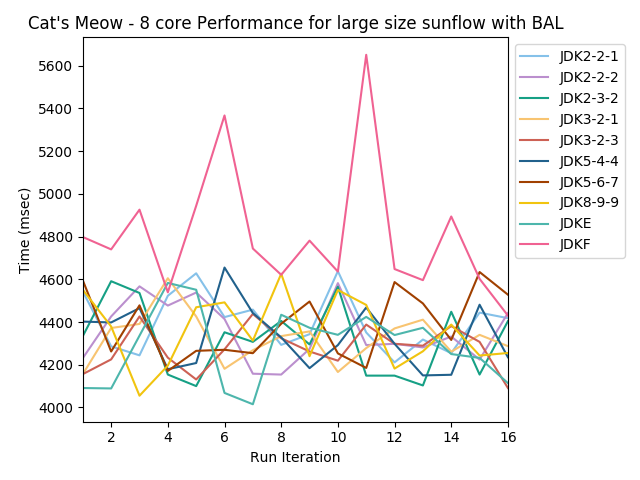
\includegraphics[width=0.8\linewidth, height=9cm]{HonoursReportTemplate_LaTeX/images/graphs/circling-8core-terminal/terminal-large-BAL-8core-sunflow.png}
       \caption{Performance time for \emph{sunflow} with Balanced}
\end{subfigure}
 \begin{subfigure}{1\textwidth}
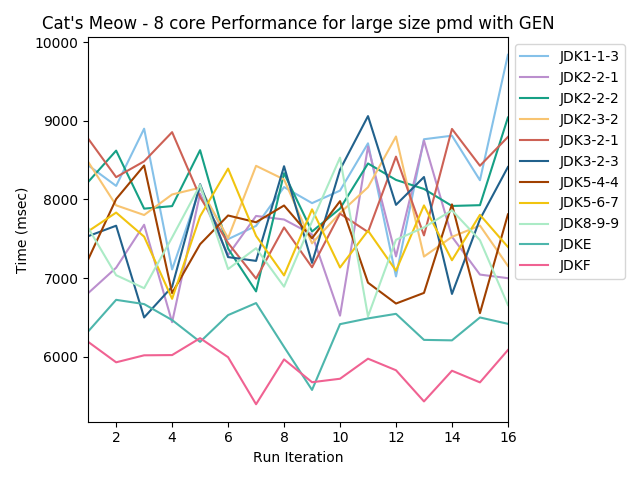
\includegraphics[width=0.8\linewidth, height=9cm]{HonoursReportTemplate_LaTeX/images/graphs/circling-8core-terminal/terminal-large-GEN-8core-pmd.png}
       \caption{Performance time for \emph{pmd} with GenCon}
\end{subfigure}

\caption{Performance for large sized benchmarks on 8-CPU machine with \emph{Circling} }
\end{figure}
\newpage
\begin{figure}[H]
\begin{subfigure}{1\textwidth}
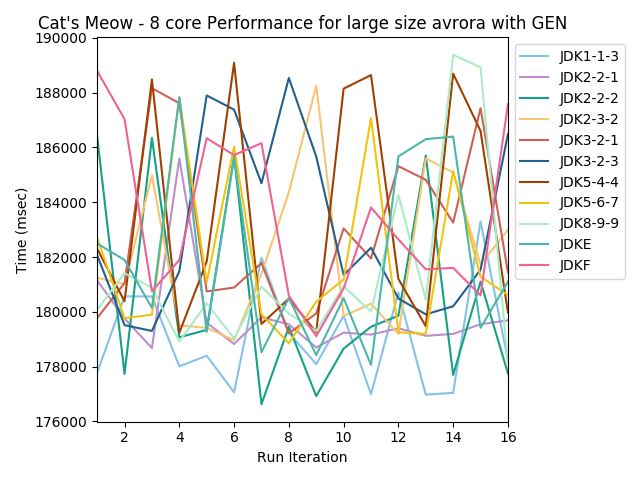
\includegraphics[width=0.8\linewidth, height=9cm]{HonoursReportTemplate_LaTeX/images/graphs/circling-8core-terminal/terminal-large-GEN-8core-avrora.png}
       \caption{Performance time for \emph{avrora} with GenCon}
\end{subfigure}

\begin{subfigure}{1\textwidth}
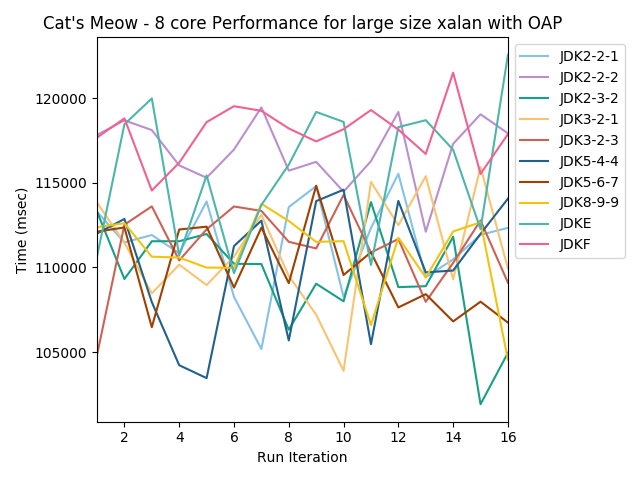
\includegraphics[width=0.8\linewidth, height=9cm]{HonoursReportTemplate_LaTeX/images/graphs/circling-8core-terminal/terminal-large-OAP-8core-xalan.png}
       \caption{Performance time for \emph{xalan} with OptAvgPause}
\end{subfigure}

    \caption{Performance for large sized benchmarks on 8-CPU machine with \emph{Circling} (1)}
    \label{fig:Circling-performance}
\end{figure}
\newpage
Based on the results from the testing conducted, it is clear that there
is a benefit to using the \emph{Circling} approach. The benefit is more
noticeable in longer-executing applications, particularly benchmarks
combined with policies that do not minimise pause times. However, the
PID controller appears to improve performance more so than GC
utilisation. Nevertheless, \emph{Circling} is an improvement over
\emph{CatNap}, naive threshold-based approach.

\subsection{Summary}
Using a PID controller provides performance benefits for applications
that do not have short execution times. There is some improvement in GC
utilisation with the PID controller implemented, but it is not
consistent. This research aims to manage GC utilisation and, thereby,
reduce the resource-intensiveness of GC. Hence, a different approach is
needed to manage GC utilisation better as the PID controller is not as
effective as expected. The next chapter discusses a \emph{Linear-Quadratic
Regulator} (LQR) and the impact of using an LQR on GC utilisation.
